%! Author = abenjeddou
%! Date = 29/06/2026

\section{Introduction}
After completing the study, design, and architecture of our system, we will move on to the implementation of the elaborated concepts.
We will delve into the implementation of our solution, detailing the different stages of setting up our architecture, while presenting the technological choices.

\section{Development environment}

\subsection{Software environment}
This section is dedicated to listing all the software and tools used throughout the project implementation.

\begin{itemize}
    \item[-] \textbf{IntelliJ IDEA}~\cite{Intel}, is an integrated development environment designed for software development based on Java technology.
    \item[-] \textbf{Minikube}~\cite{minikube}, is an open-source tool that facilitates setting up a local Kubernetes cluster on your machine. It allows developers to test, develop, and deploy Kubernetes applications without requiring a full Kubernetes cluster infrastructure.
    \item[-] \textbf{Docker-cli}, is the command-line interface that allows users to interact with Docker. It enables users to perform a variety of tasks related to managing containers, images, networks, and Docker volumes.
    \item[-] \textbf{Kubectl}, is a Kubernetes command-line tool. It allows executing commands in Kubernetes clusters. It is used to deploy applications, inspect and manage cluster resources, and view logs.
    \item[-] \textbf{Helm}~\cite{helm}, is an open-source package management tool for Kubernetes. It simplifies and automates the deployment of applications and services on Kubernetes clusters using configuration files called charts.
\end{itemize}

\subsection{Technologies}

\begin{itemize}
    \item[-] \textbf{Flink}~\cite{FLINK}, is a real-time data processing and large-scale batch processing system. It is an open-source project developed by the Apache Foundation, designed to offer high availability, low latency, and high data stream processing capacity.
    \item[-] \textbf{Kubernetes}~\cite{K8S}, is an extensible and portable open-source platform for managing containerized workloads and services. It promotes both declarative configuration and automation. It is a large, rapidly expanding ecosystem. Kubernetes services, support, and tools are widely available.
    \item[-] \textbf{Docker}~\cite{docker}, is a virtualization technology that allows running applications in containers.
    \item[-] \textbf{Syslog}, is a standard protocol used for collecting and transmitting logs across the network.
    \item[-] \textbf{ELK}~\cite{elk}, Elasticsearch is the log storage engine enabling fast search and analysis. Logstash is often used to normalize and enrich logs before they are stored in Elasticsearch. Kibana is used as a user interface to explore and visualize data stored in Elasticsearch.
    \item[-] \textbf{Prometheus}~\cite{prometheus}, is an open-source tool developed by SoundCloud in 2012. It enables monitoring of systems, servers, applications, and other infrastructure. It relies on a time-series database to supervise, track events, and manage alerts.
    \item[-] \textbf{Grafana}~\cite{grafana}, is a powerful data visualization and monitoring tool. It provides real-time dashboards and graphs on application and service performance and metrics.
    \item[-] \textbf{GitLab}, is a DevOps software suite that combines the ability to develop, secure, and operate software in a single application. The open-source software project was created by Ukrainian developer Dmitriy Zaporozhets and Dutch developer Sytse Sijbrandij. Since its creation, GitLab has been focused on remote work. GitLab is the largest fully remote company in the world, with approximately 30 million registered users, including 1 million active licensed users.
    \item[-] \textbf{RabbitMQ}~\cite{RBMQ}, is an open-source messaging software designed to manage communication between distributed applications. It uses the AMQP standard to transfer messages between applications.
\end{itemize}

\section{Flink job implementation}

\subsection{Job workflow}
Figure 4.1 details the different stages of a message's journey before being transmitted to the Erable API.
Our Flink job continuously consumes messages from RabbitMQ, connecting to a queue where events arrive continuously.
It then proceeds with JSON conversion.
The next step is to validate the message format against a previously defined Avro schema.
If the message does not conform, it is rejected, and processing moves to the next message.

Subsequently, we retrieve the subscription from the Valkey API by making a request with the client identifier.
We then enrich the message with information such as the device on which the notification will be received.

Before sending the message to the Erable API, which is responsible for dispatching notifications to the client, we must update the notification date in the client's subscription by querying the Valkey API.

\begin{center}
    \centering
    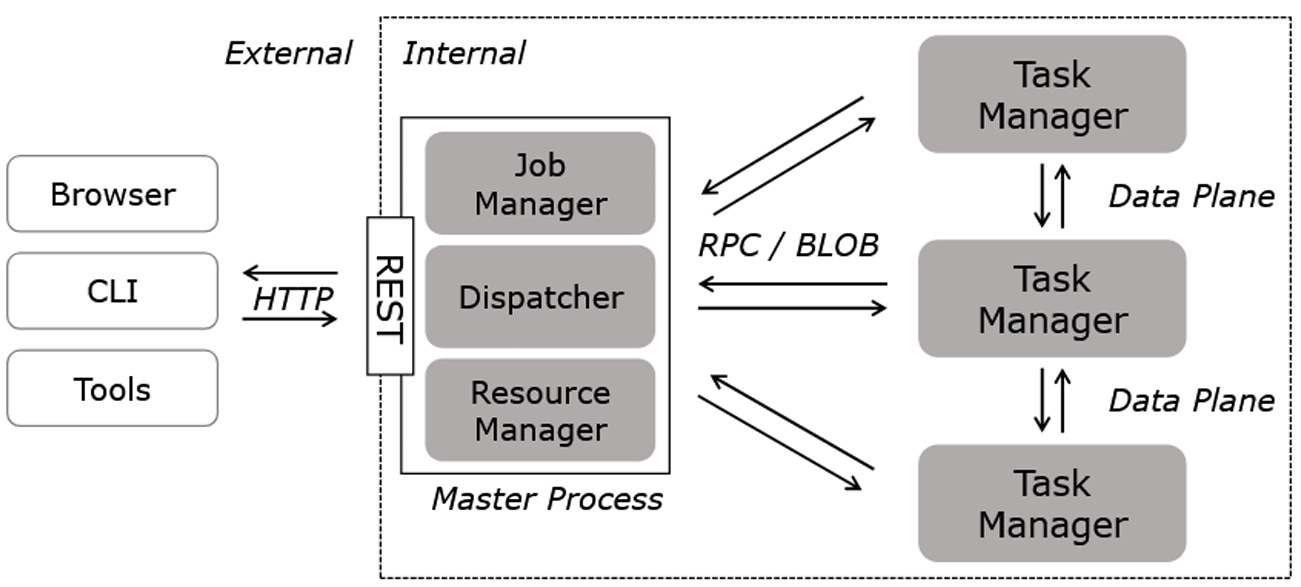
\includegraphics[width=0.9\textwidth]{img/flink_connectivity}
    \captionof{figure}{Flink job workflow}
\end{center}

\subsection{Job visualization}
Figure 4.2 illustrates the Flink user interface.
In this view, we can observe elements such as the current job status and the available Task Managers for deploying the different tasks.
This interface provides real-time visibility into the operation of our deployed Flink job, thus facilitating monitoring and troubleshooting.

\begin{center}
    \centering
    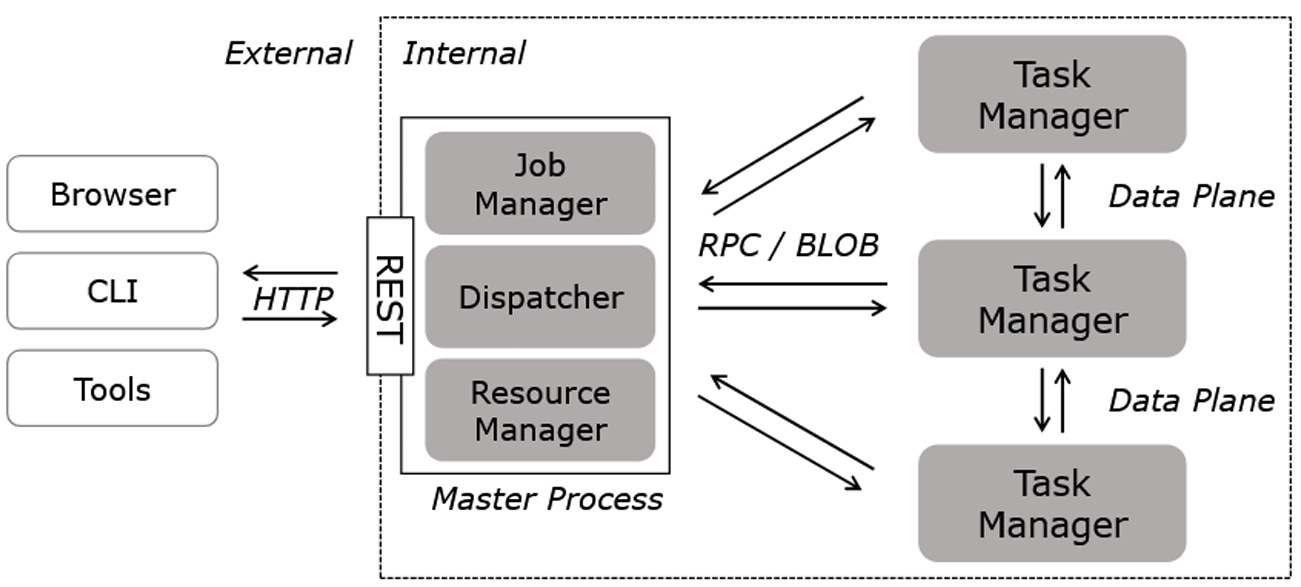
\includegraphics[width=0.9\textwidth]{img/flink_connectivity}
    \captionof{figure}{Flink user interface}
\end{center}

Figure 4.3 represents the Flink job topology, illustrating how the different components of the job interact with each other to process data.
More specifically, it shows the data path through the different operations of our job, from the initial source to the final destination.

\begin{center}
    \centering
    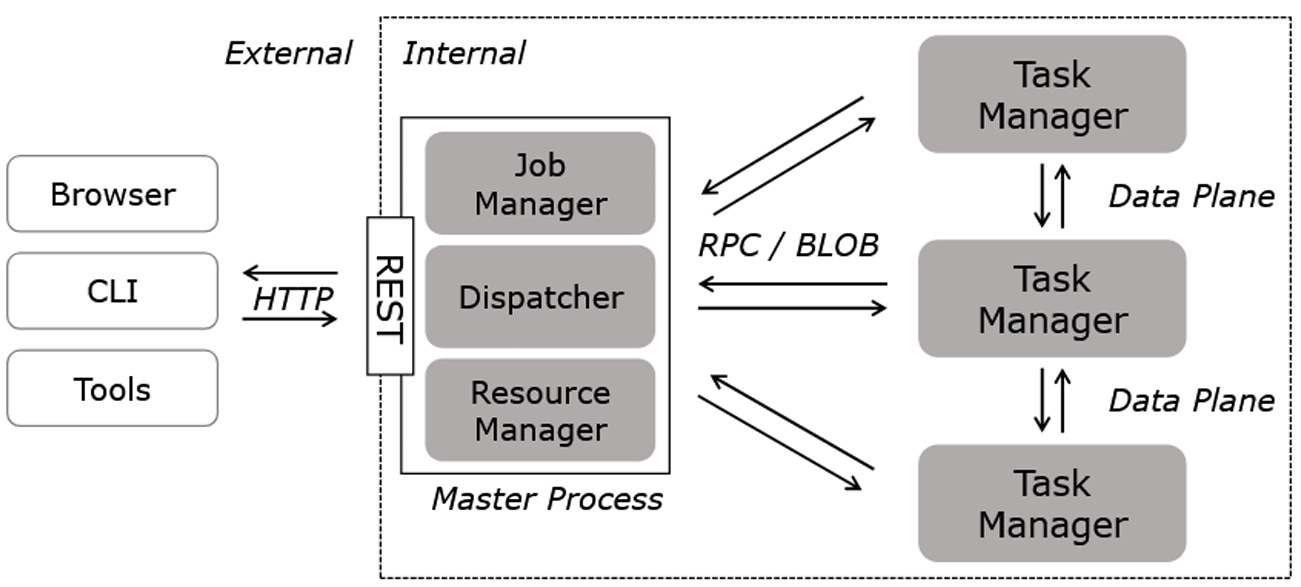
\includegraphics[width=0.9\textwidth]{img/flink_connectivity}
    \captionof{figure}{Job topology}
\end{center}

Figure 4.4 offers a detailed overview of the different deployed operators, the data processed and exchanged between them, as well as their deployment statuses.
We notice that each operator is deployed twice due to the job's parallelism, which is set to 2.
This allows us to understand the entire data flow and identify the stages where transit issues were encountered.

\subsection{AI Model Implementation}

\subsubsection{Dataset}

The AI model is trained on historical fair-use notification data collected from the production pipeline.
Each data point represents a single fair-use event received from the DCB (Data Consumption Broker) system,
enriched with subscription state information stored in Valkey.

\paragraph{Data Sources}
\begin{itemize}
    \item[-] \textbf{FairUse events} from the RabbitMQ~\cite{RBMQ} queue (RMQ\_LFU\_QUEUE): contain the MSISDN,
    customer type, event type, reached threshold percentage, and event date.
    \item[-] \textbf{Subscription state} from Valkey (LfuMainRecord): contains the historical
    notification state, including the timestamp of the last notification sent per event type.
\end{itemize}

Each sample is labeled with whether a quota overshoot actually occurred within the billing cycle
(binary label: overshoot / no overshoot).

\subsubsection{Features}

The model uses \textbf{7 engineered features}, extracted by the PredictionFeatureExtractor class.
All features are normalized to the $[0, 1]$ range.

\begin{table}[htbp]
    \justifying
    \centering
    \begin{tabularx}{\textwidth}{|p{2.5cm}|p{3.5cm}|X|}
        \hline
        \textbf{Feature} & \textbf{Encoding} & \textbf{Rationale} \\
        \hline
        Reached Threshold \% & $\frac{\text{value}}{100}$ &
        Direct indicator of quota consumption level.
        Higher values signal imminent overshoot. \\
        \hline
        Customer Type & GP$=$0.0, ENT$=$0.5, MVNO$=$1.0 &
        Different customer segments exhibit different consumption patterns. \\
        \hline
        Hour of Day & $\frac{\text{hour}}{23}$ &
        Captures intra-day consumption patterns (peak hours vs.\ nighttime).
        Timezone: Europe/Paris. \\
        \hline
        Day of Week & $\frac{\text{dayOfWeek} - 1}{6}$ &
        Captures weekly seasonality (weekday vs.\ weekend consumption). \\
        \hline
        Hours Since Last Notification & $\frac{\text{hours}}{720}$ (capped at 30 days) &
        Measures notification recency. Short interval indicates rapid consumption. Defaults to 1.0 if no prior state. \\
        \hline
        Day in Billing Cycle & $\frac{\text{dayOfMonth} - 1}{\text{daysInMonth} - 1}$ &
        Critical contextual feature. Reaching 80\% on day~5 ($\approx$0.13) is far more alarming than on day~28 ($\approx$0.90), because billing resets on the 1\textsuperscript{st} of each month. \\
        \hline
        Event Type & fairuse$=$0.0, blocage$=$0.25, redirect$=$0.5, alerting$=$0.75, leveeFU$=$1.0 &
        Encodes event severity. Blocking/redirect events carry higher risk. \\
        \hline
    \end{tabularx}
    \caption{Feature description}
    \label{tab:features}
\end{table}

\subsubsection{Model}

\paragraph{Algorithm}

The model is a \textbf{binary classifier} exported in \textbf{ONNX format}~\cite{onnx},
loaded at runtime via the ONNX Runtime Java API~\cite{onnxruntime} (AI.onnxruntime).
The ONNX format enables framework-agnostic deployment: the model can be trained in Python (scikit-learn~\cite{sklearn}, XGBoost~\cite{xgboost}, PyTorch, etc.)
and served natively in the JVM without Python dependencies.

The recommended algorithm is a \textbf{Gradient Boosted Decision Tree (GBDT)}, such as XGBoost or LightGBM,
well-suited for:
\begin{itemize}
    \item[-] Tabular data with mixed feature types;
    \item[-] Small to medium feature space (7~features);
    \item[-] High interpretability requirements (feature importance analysis);
    \item[-] Low-latency inference in streaming contexts.
\end{itemize}

A \textbf{rule-based fallback} is automatically activated when the ONNX model is unavailable (missing file or loading error).
The fallback uses the following weighted heuristic:

\begin{multline}
    \text{score} = 0.35 \times \text{thresholdRisk}
    + 0.25 \times \underbrace{\text{thresholdRisk} \times (1 - \text{billingCyclePosition})}_{\text{urgencyFactor}} \\
    + 0.20 \times \text{recencyRisk}
    + 0.20 \times \text{eventRisk} \\
\end{multline}

This fallback encodes the key domain insight: high quota usage early in the billing cycle is
exponentially more dangerous than the same usage near the end of the cycle.

\paragraph{Training}

The training pipeline (offline, in Python) follows these steps:

\begin{enumerate}
    \item \textbf{Data collection}: Historical fair-use events and their outcomes (overshoot within
    the billing cycle) are extracted from Valkey and the notification logs.
    \item \textbf{Feature engineering}: The same 7~features defined in PredictionFeatureExtractor
    are computed for each training sample to ensure consistency between training and inference.
    \item \textbf{Train/validation/test split}: 70\% / 15\% / 15\% stratified split to preserve
    class balance (overshoot events are relatively rare).
    \item \textbf{Hyperparameter tuning}: Grid search or Bayesian optimization over key parameters
    (max\_depth, learning\_rate, n\_estimators, min\_child\_weight).
    \item \textbf{Export}: The trained model is exported to ONNX format via skl2onnx or
    onnxmltools and embedded in the Flink~\cite{FLINK} job container at
    /models/fairuse\_prediction.onnx.
\end{enumerate}

\paragraph{Evaluation}

The model is evaluated on the held-out test set using the metrics described in Table~\ref{tab:metrics}.

\begin{table}[htbp]
    \justifying
    \centering
    \begin{tabularx}{\textwidth}{|l|X|c|}
        \hline
        \textbf{Metric} & \textbf{Description} & \textbf{Target} \\
        \hline
        Accuracy &
        Overall correct predictions / total predictions. &
        $\geq 90\%$ \\
        \hline
        Precision &
        $\frac{TP}{TP + FP}$. Measures how many flagged overshoots are real.
        High precision avoids unnecessary notifications to customers. &
        $\geq 85\%$ \\
        \hline
        Recall &
        $\frac{TP}{TP + FN}$. Measures how many actual overshoots are caught.
        High recall ensures no customer is surprised by unexpected quota exhaustion. &
        $\geq 80\%$ \\
        \hline
        F1-Score &
        Harmonic mean of precision and recall: $\frac{2 \times P \times R}{P + R}$.
        Balances the trade-off between false alarms and missed detections. &
        $\geq 82\%$ \\
        \hline
        RMSE &
        Root Mean Squared Error on the prediction score (continuous output $[0, 1]$).
        Measures calibration quality---how well the predicted probability matches the
        actual overshoot frequency. &
        $\leq 0.15$ \\
        \hline
        AUC-ROC &
        Area Under the ROC Curve. Measures discrimination ability across all thresholds. &
        $\geq 0.92$ \\
        \hline
    \end{tabularx}
    \caption{Model evaluation metrics and targets}
    \label{tab:metrics}
\end{table}

\subsubsection{Runtime Metrics (Flink)}

The following counters are exposed in real-time via the Flink metrics system
(Table~\ref{tab:runtime-metrics}).

\begin{center}
    \justifying
    \begin{tabularx}{\textwidth}{|l|c|X|}
        \hline
        \textbf{Metric} & \textbf{Group} & \textbf{Description} \\
        \hline
        predictions\_total & ai &
        Total number of predictions performed. \\
        \hline
        anomalies\_detected & ai &
        Number of messages flagged as anomalous (score $\geq$ AI\_ANOMALY\_THRESHOLD, default 0.85). \\
        \hline
        fallback\_used & ai &
        Number of predictions made using the rule-based fallback (model unavailable). \\
        \hline
    \end{tabularx}
    \captionof{table}{Flink runtime AI metrics}
    \label{tab:runtime-metrics}
\end{center}

\subsubsection{Configuration}

\begin{center}
    \justifying
    \begin{tabularx}{\textwidth}{|p{4cm}|p{4cm}|X|}
        \hline
        \textbf{Environment Variable} & \textbf{Default} & \textbf{Description} \\
        \hline
        AI\_ANOMALY\_ THRESHOLD & 0.85 &
        Score threshold above which a consumption pattern is flagged as anomalous. \\
        \hline
        AI\_MODEL\_ PATH & /models/fairuse\_ prediction.onnx &
        Classpath location of the ONNX model file. \\
        \hline
    \end{tabularx}
    \captionof{table}{AI configuration environment variables}
    \label{tab:ai-config}
\end{center}

\subsubsection{Resilience}

The AI prediction step is designed to be \textbf{non-blocking}: if prediction fails for any reason
(model loading error, inference exception), the message is still forwarded downstream with a
predictionScore of $-1.0$, ensuring the core notification pipeline is never interrupted
by the AI component.

\section{Deployment on Kubernetes}

\subsection{Deployment environment}
RicKaaStley is a CaaS (Container as a Service) whose purpose is to offer a shared and multi-tenant hosting solution for containerized applications.
It is both a hosting platform and a set of operational services provided on this platform: capabilities to manage metrics, logs, and container orchestration.
The orchestration technology is Kubernetes.

RicKaaStley provides computing resources: CPU, RAM, Network, and Storage, as well as secure, isolated, and sealed environments for each of its clients (who consume these resources through their applications).
It is therefore a shared and multi-tenant service, meaning that RicKaaStley serves multiple clients isolated from one another: they cannot see each other, do not interact in their consumption of the service, and each is guaranteed the ability to use the resources contracted during subscription.

\subsection{Deployment with Helm}
To deploy our Flink job, we chose to use Helm~\cite{helm} to simplify the lifecycle management of our Flink job.
Helm groups all the YAML files required for deploying our various cluster components into a package called a Chart.

\subsection{Helm chart management}

\subsubsection{Installation}
Figure 4.5 shows the Helm command that installs the chart located in the ``chart/'' directory, using a default values file as well as a values file specific to the internal environment.
This allows deploying our Flink job with environment-specific configurations while maintaining flexibility through value file customization.

\begin{center}
    \centering
    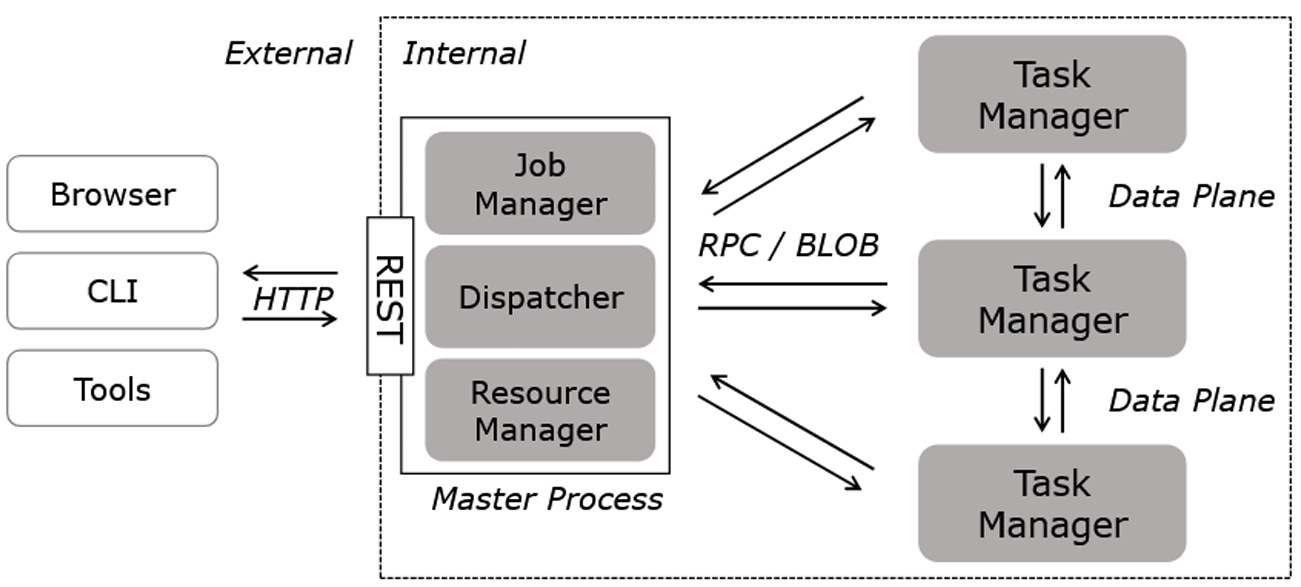
\includegraphics[width=0.9\textwidth]{img/flink_connectivity}
    \captionof{figure}{Helm chart installation}
\end{center}

\subsubsection{Helm chart uninstallation}
Figure 4.6 illustrates the Helm command that uninstalls our Flink job named ``send-notif'' from the Kubernetes cluster.
This involves stopping and removing all components deployed by the Helm chart associated with this installation.

\begin{center}
    \centering
    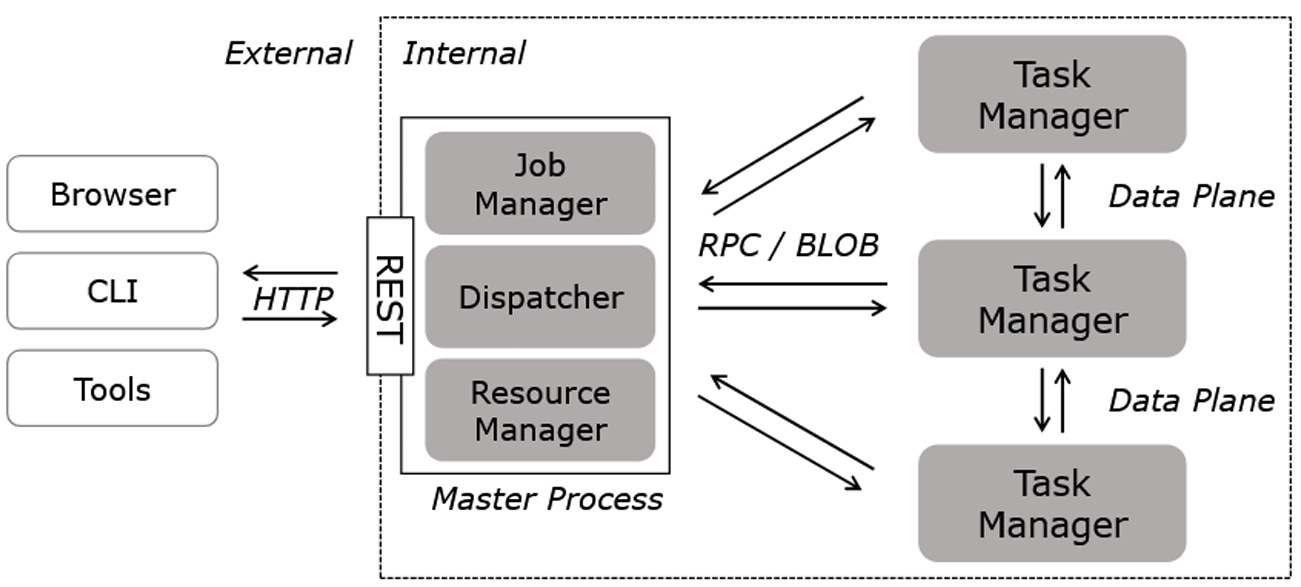
\includegraphics[width=0.9\textwidth]{img/flink_connectivity}
    \captionof{figure}{Helm chart uninstallation}
\end{center}

\subsection{Deployed resources}
Figure 4.7 highlights the Kubernetes resources deployed by the Helm chart.
The chart consists of a set of files describing the resources of a Kubernetes cluster.

\begin{center}
    \centering
    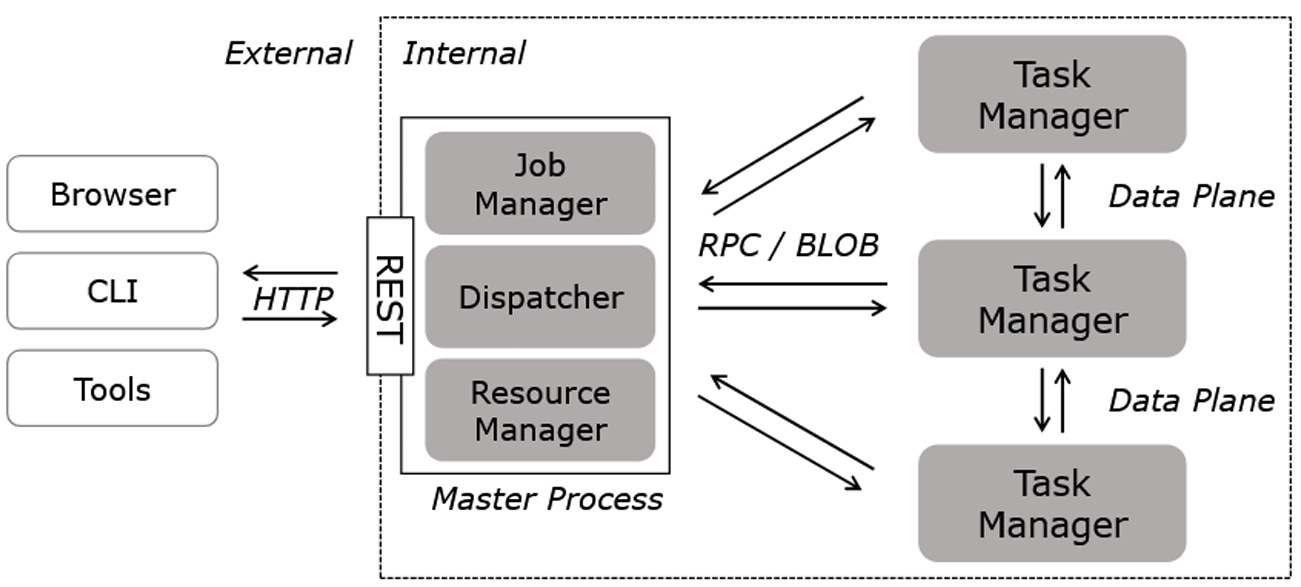
\includegraphics[width=0.9\textwidth]{img/flink_connectivity}
    \captionof{figure}{Deployment architecture}
\end{center}

Our chart deploys the following resources:

\begin{itemize}
    \item[-] \textbf{A Kubernetes Job object:} manages the JobManager.
    \item[-] \textbf{A Kubernetes Deployment object:} manages the TaskManagers.
    \item[-] \textbf{A Flink-UI service:} exposes the Flink graphical interface to users.
    \item[-] \textbf{A Prometheus service:} exposes metrics so they can be consumed by Prometheus.
    \item[-] \textbf{A ConfigMap:} contains the configuration of our Flink job and will be injected as a YAML file.
\end{itemize}

\section{Taking a savepoint}
A savepoint is a consistent image of the execution state of a stream processing task, created using Flink's checkpointing mechanism.
We can use savepoints to stop and resume or update our Flink jobs.
Savepoints consist of two parts: a directory with binary files (usually large) stored in stable storage (e.g., HDFS, S3, ...) and a metadata file (relatively small).
The stable storage files represent the net data of the job execution state image.
The savepoint metadata file mainly contains pointers to all the stable storage files that are part of the savepoint, in the form of relative paths.

Figure 4.13 shows the command that allows us to retrieve the Flink job ID in order to use it to take a savepoint.

\begin{center}
    \centering
    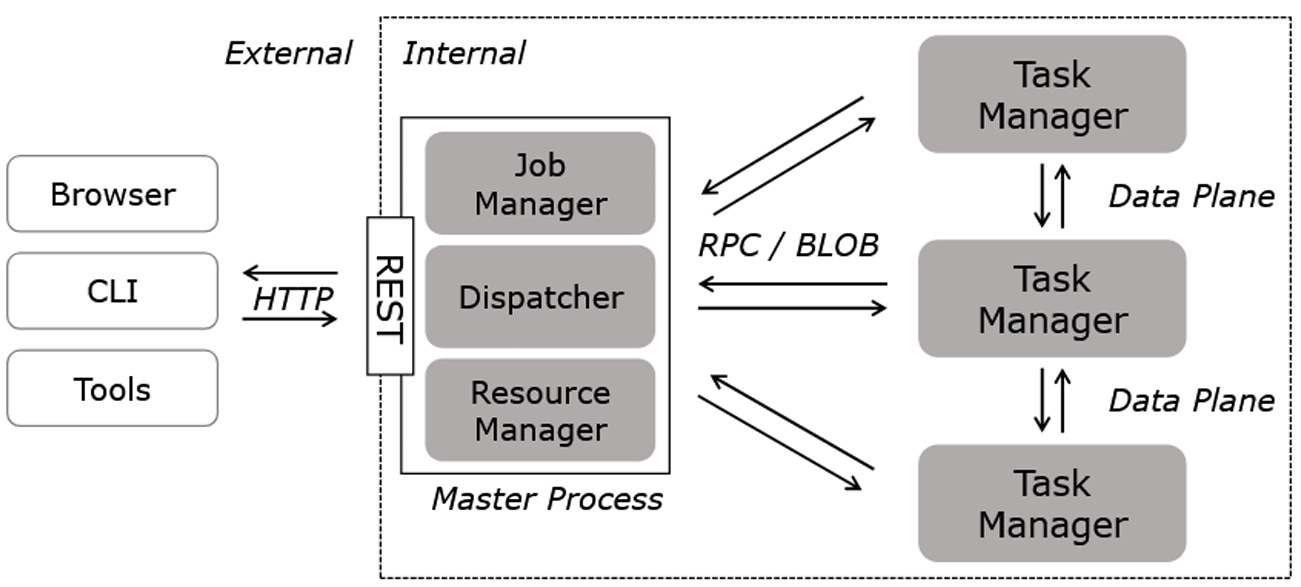
\includegraphics[width=0.9\textwidth]{img/flink_connectivity}
    \captionof{figure}{Displaying the job ID}
\end{center}

Figure 4.14 shows the command for taking a savepoint and storing it on Amazon S3.
This savepoint can then be used to restart the job later after making some configurations or a version update.

\begin{center}
    \centering
    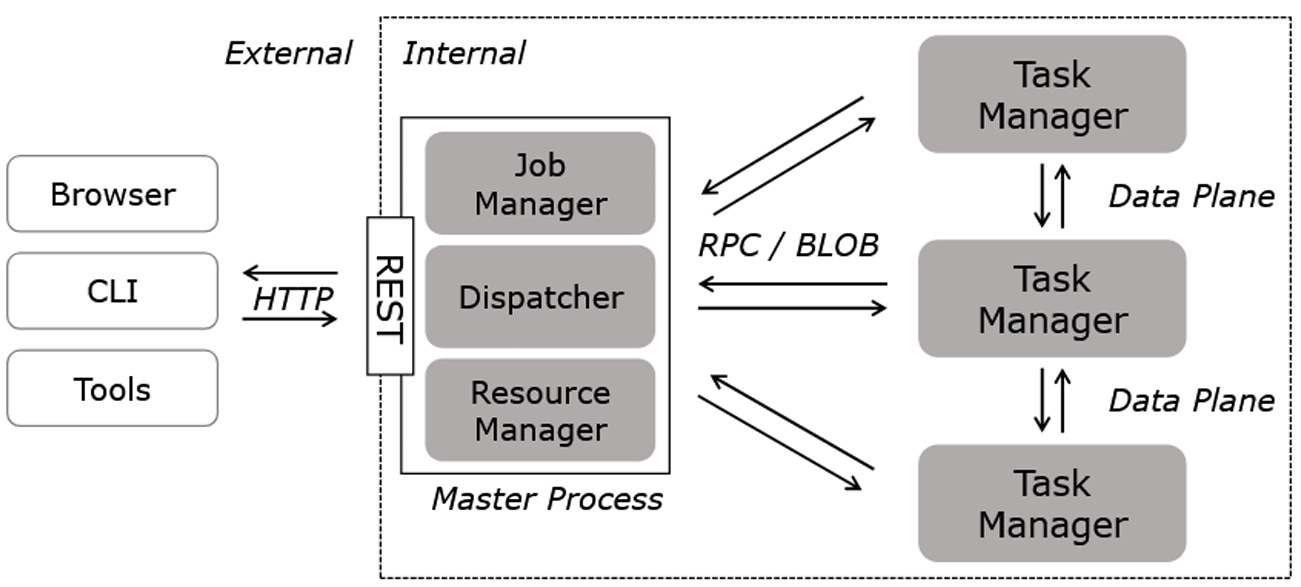
\includegraphics[width=0.9\textwidth]{img/flink_connectivity}
    \captionof{figure}{Taking a savepoint}
\end{center}

\section{RabbitMQ data source}
RabbitMQ~\cite{RBMQ} plays a central role as the primary data source for our Flink job.
The current RabbitMQ queue configuration, shown in Figure 4.15, establishes a crucial link with our Flink job, ensuring a continuous and smooth data flow towards real-time processing.
The presence of two consumers connected to the queue clearly illustrates the connection between our Flink job and the queue.
Additionally, our queue is connected to an exchange on which messages arrive and are routed to the queue as illustrated in Figure 4.16.

It is important to note that the connection to RabbitMQ is made via the secure AMQPS protocol.
The use of this protocol guarantees a secure connection, thus reinforcing the reliability and confidentiality of data exchanges between RabbitMQ and our Flink job.
This secure approach helps ensure data integrity throughout the process.

\begin{center}
    \centering
    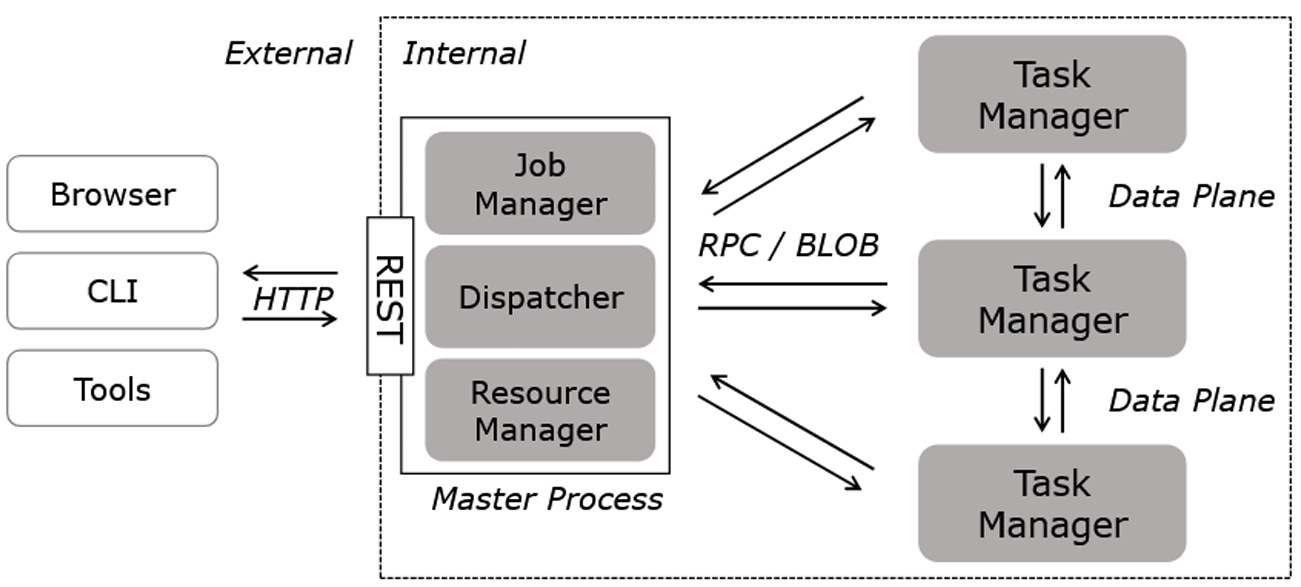
\includegraphics[width=0.9\textwidth]{img/flink_connectivity}
    \captionof{figure}{The RabbitMQ queue}
\end{center}

\begin{center}
    \centering
    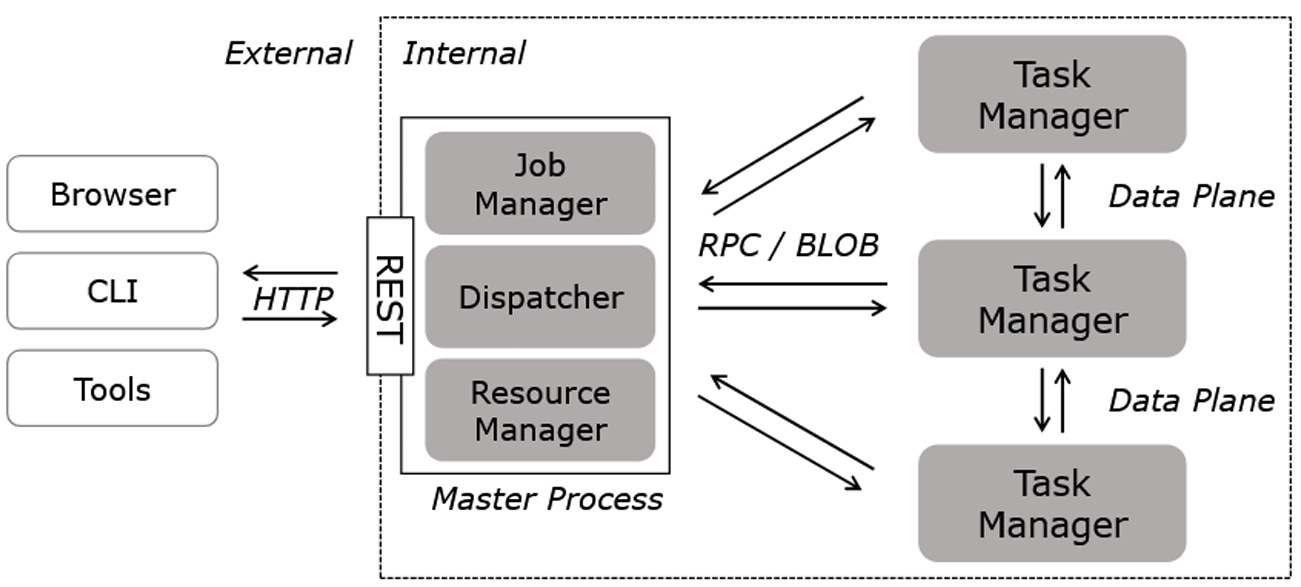
\includegraphics[width=0.9\textwidth]{img/flink_connectivity}
    \captionof{figure}{The RabbitMQ exchange}
\end{center}

\section{Message processing scenario}
The message is sent to the exchange, which in turn routes it to the queue.
As soon as the message reaches the queue, it is consumed by Flink, as shown in Figure 4.17, by observing the RabbitMQ graphical interface.

\begin{center}
    \centering
    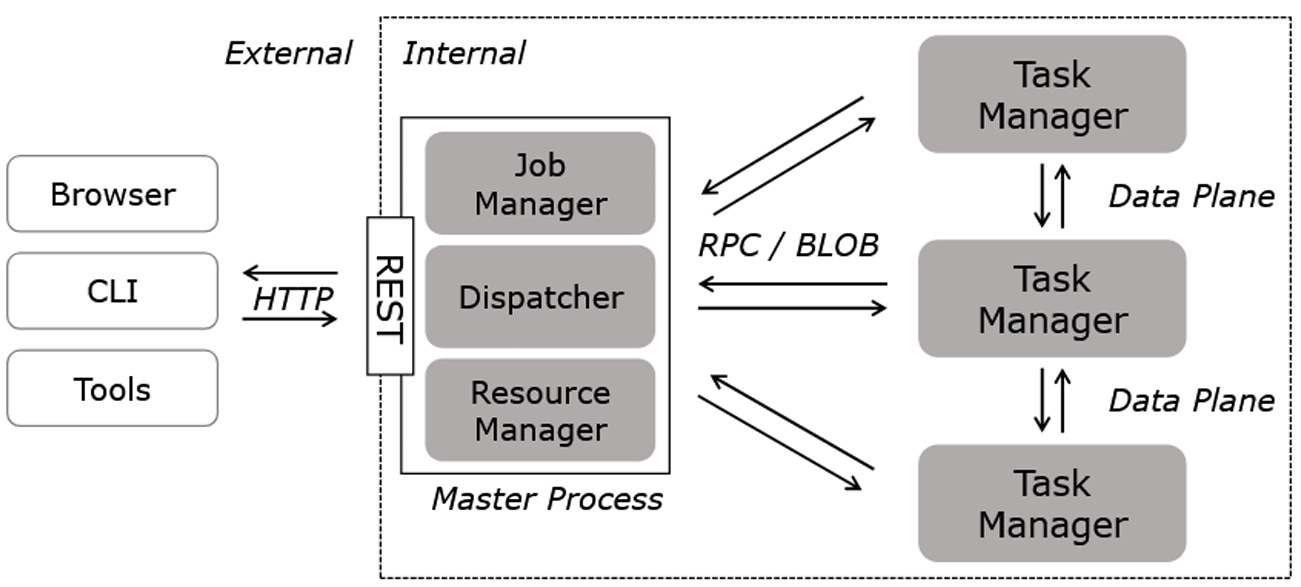
\includegraphics[width=0.9\textwidth]{img/flink_connectivity}
    \captionof{figure}{Sending a message to RabbitMQ}
\end{center}

Figure 4.18 clearly illustrates the logs on the TaskManager confirming that the message was properly processed, arriving at the final step which consists of sending the message to the Erable API.

\begin{center}
    \centering
    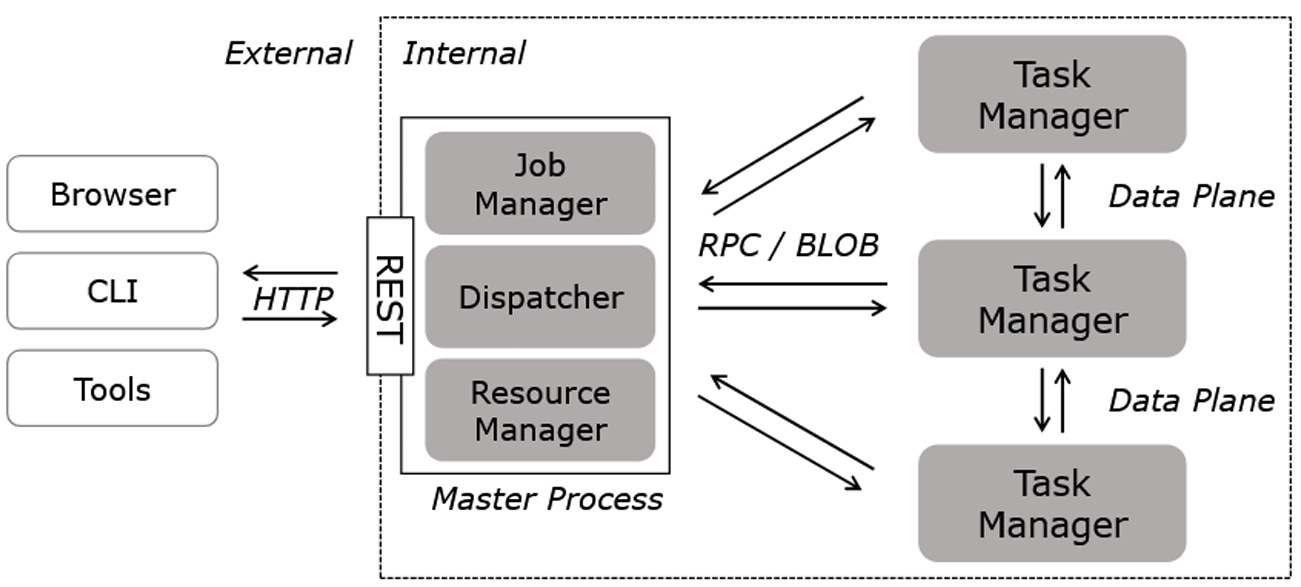
\includegraphics[width=0.9\textwidth]{img/flink_connectivity}
    \captionof{figure}{Logs on the TaskManager}
\end{center}

Figure 4.19 shows us the trace, on Kibana, of our message processing by the Flink job.

\begin{center}
    \centering
    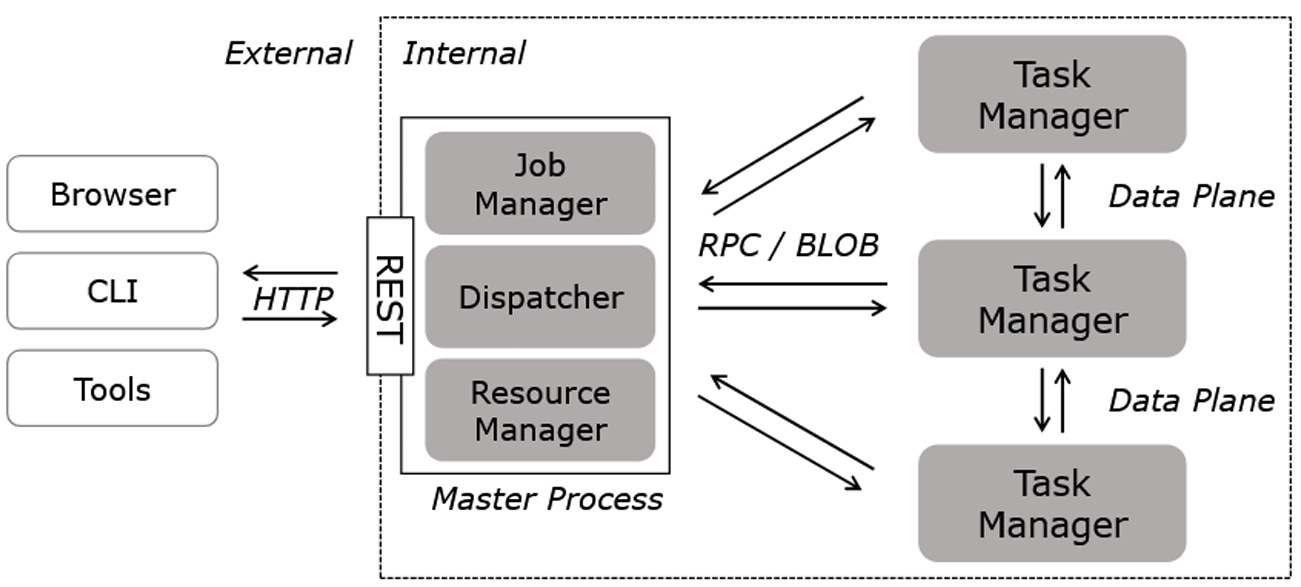
\includegraphics[width=0.9\textwidth]{img/flink_connectivity}
    \captionof{figure}{Logs on Kibana}
\end{center}

By consulting the Flink user interface, we observe an increase in the number of messages, thus confirming that the message was received and processed by our Flink job as illustrated in Figure 4.20.

\begin{center}
    \centering
    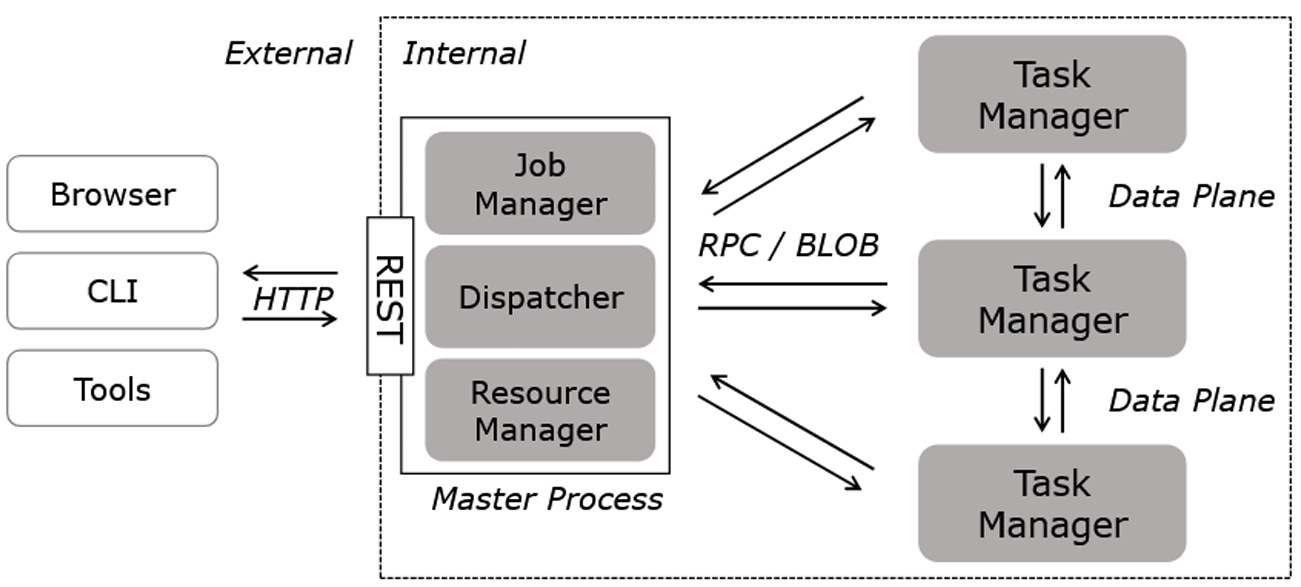
\includegraphics[width=0.9\textwidth]{img/flink_connectivity}
    \captionof{figure}{Message processing trace on the Flink UI}
\end{center}

Figure 4.21 confirms that the message was consumed by the Flink job, was acknowledged, and consequently disappears from RabbitMQ.

\begin{center}
    \centering
    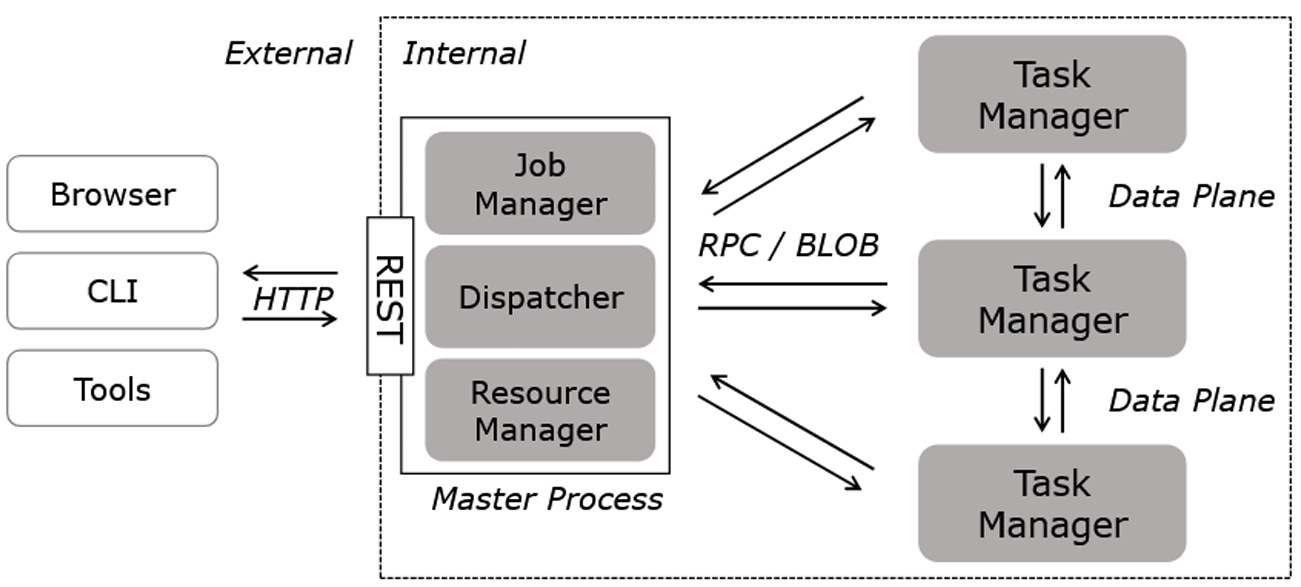
\includegraphics[width=0.9\textwidth]{img/flink_connectivity}
    \captionof{figure}{Message acknowledgment on RabbitMQ}
\end{center}

\section{Checkpoint visualization}
In the context of monitoring checkpoints in Flink, the web interface offers a dedicated tab providing detailed information about a job's checkpoints, as illustrated in Figure 4.22.
This tab presents various statistics, including the number of triggered, in-progress, completed, and failed checkpoints.
We also have the ability to examine the latest checkpoint in detail, including its total validation duration, the size of saved data, and other relevant information.
These details provide an in-depth view, thus facilitating the monitoring and efficient management of checkpoints to ensure Flink job resilience.

\begin{center}
    \centering
    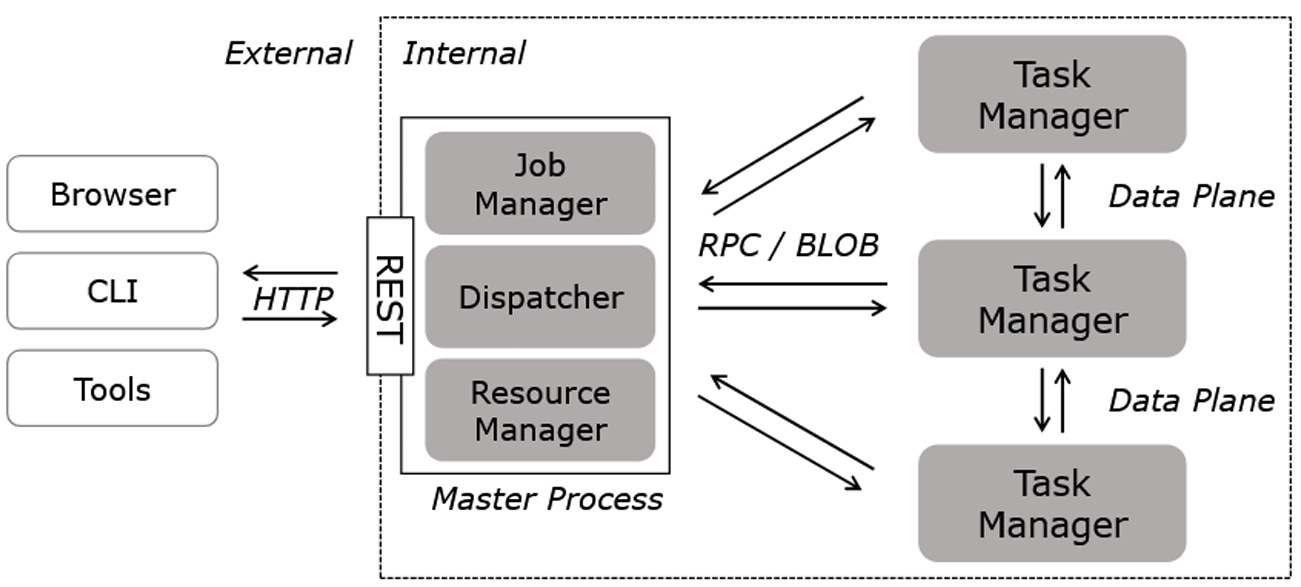
\includegraphics[width=0.9\textwidth]{img/flink_connectivity}
    \captionof{figure}{Checkpoint visualization on the Flink UI}
\end{center}

Figure 4.23 highlights the logs on the JobManager pod, demonstrating the regular execution of checkpoints.

\begin{center}
    \centering
    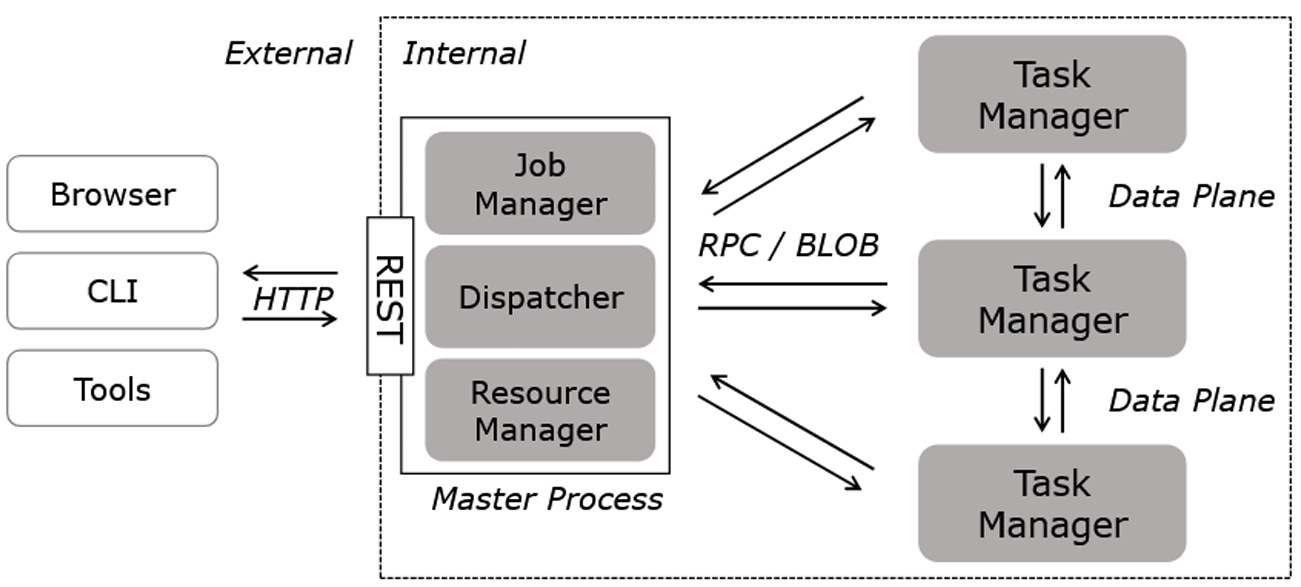
\includegraphics[width=0.9\textwidth]{img/flink_connectivity}
    \captionof{figure}{Checkpoint logs on the JobManager}
\end{center}

Figure 4.24 presents the graphical interface of Scality, a tool that provides access to our S3 buckets to visualize and manage the data stored there, allowing us to observe the last ten checkpoints saved by our Flink job.

\begin{center}
    \centering
    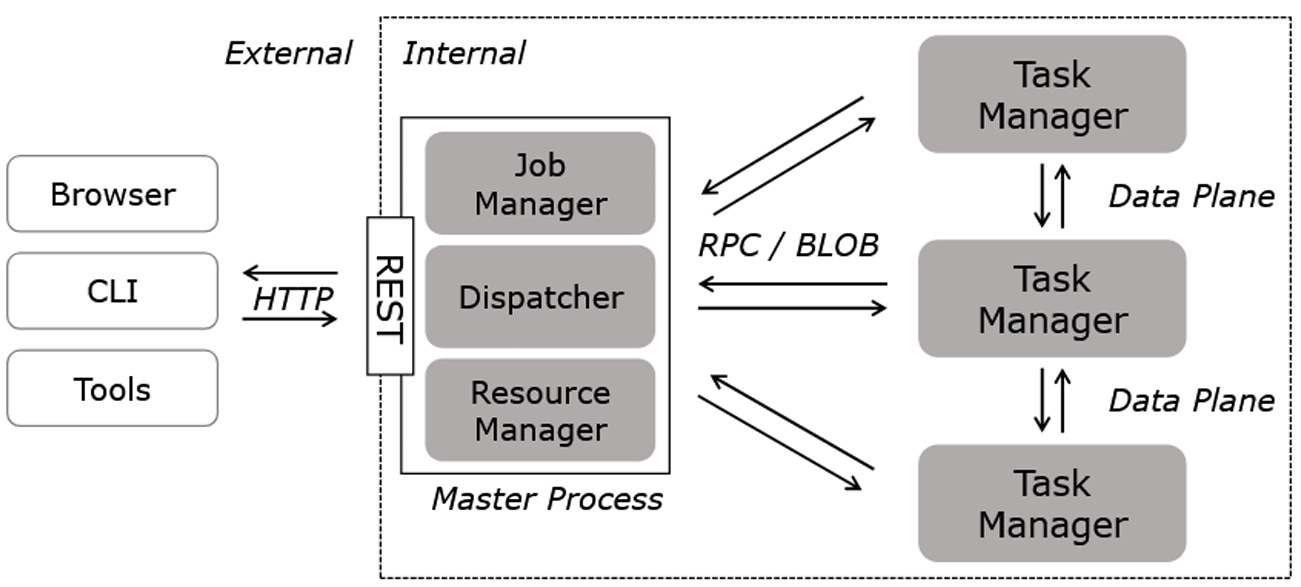
\includegraphics[width=0.9\textwidth]{img/flink_connectivity}
    \captionof{figure}{Checkpoint storage on S3}
\end{center}

\section{Log visualization}
Once our cluster is deployed, it is important to visualize logs in a centralized and clear manner to facilitate problem resolution.
It is with this in mind that we integrated the ELK~\cite{elk} stack to assist us in consulting the logs generated by our Flink job.
Using the ELK stack allows us to have a unified view of the state of our systems, thus simplifying the diagnostic process and performance improvement.

Figure 4.25 illustrates the log exploitation process.
Syslog sends logs to Logstash, which subsequently stores them in Elasticsearch.
They then become accessible for exploitation in the Kibana dashboard, enabling in-depth analyses and relevant visualizations.

\begin{center}
    \centering
    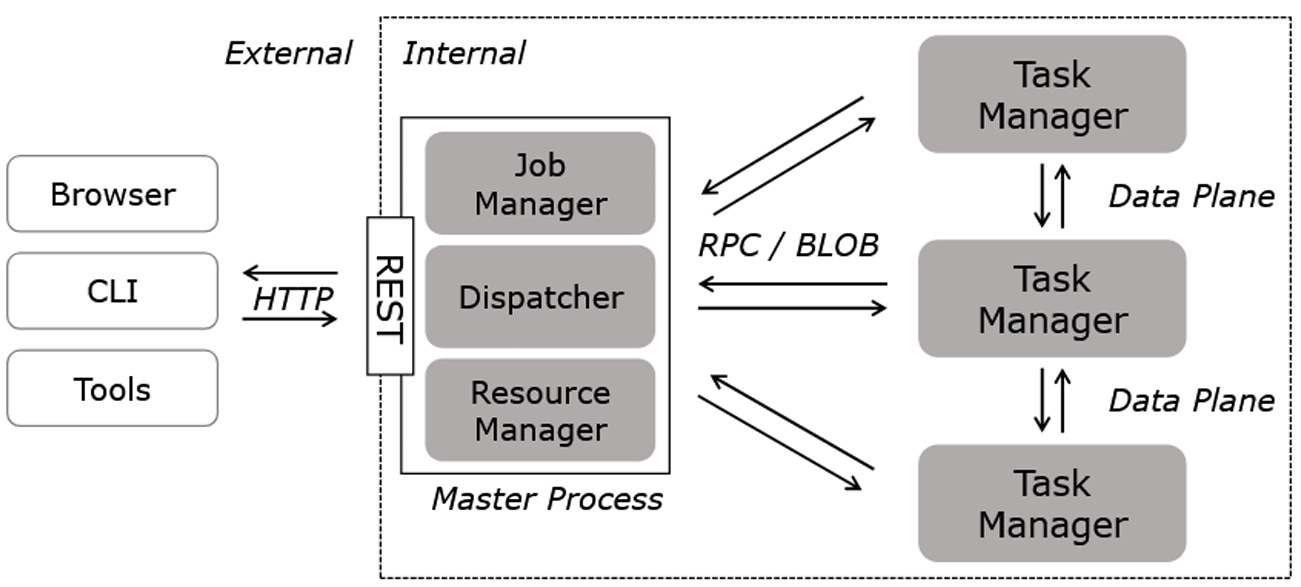
\includegraphics[width=0.9\textwidth]{img/flink_connectivity}
    \captionof{figure}{Log exploitation}
\end{center}

Thanks to Kibana, we have the ability to access the logs of our Flink job as shown in Figure 4.26, thus offering the capability to filter data or generate precise statistics over well-defined time periods.

\begin{center}
    \centering
    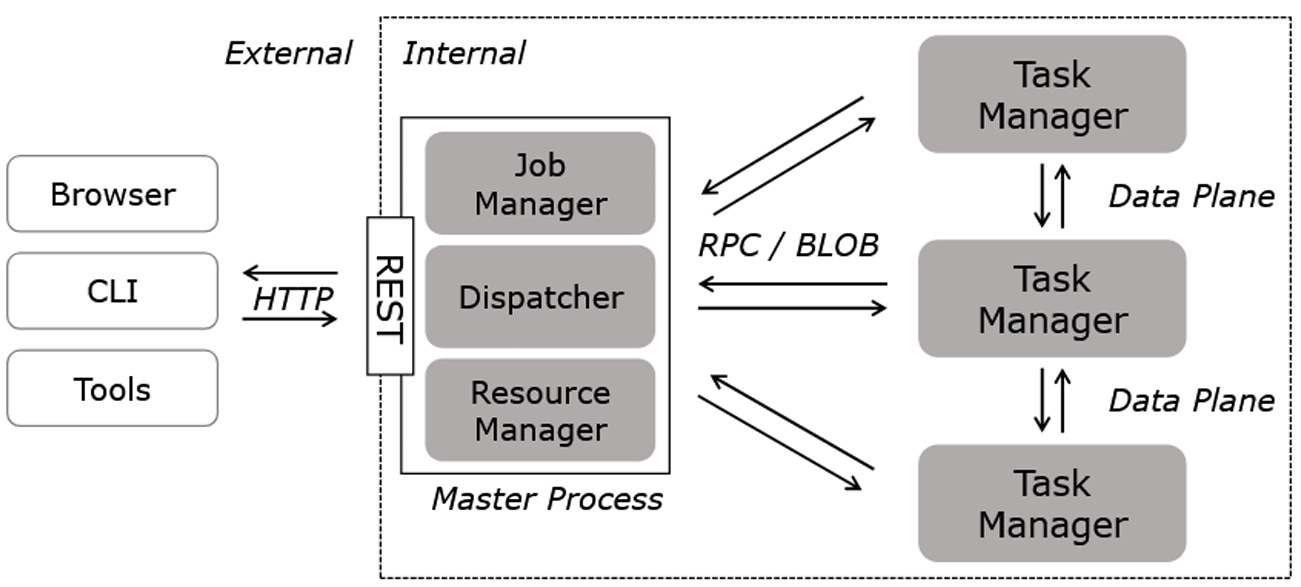
\includegraphics[width=0.9\textwidth]{img/flink_connectivity}
    \captionof{figure}{Log visualization on Kibana}
\end{center}

\section{Metrics supervision}
When our job is running, it is essential to implement rigorous monitoring by analyzing the various exposed metrics.
This approach ensures the proper functioning of the job and detects potential issues.
Among the essential aspects of monitoring is memory, which receives particular attention.

Figure 4.27 illustrates the operation of the supervision component.
Prometheus~\cite{prometheus} collects metrics from our Flink job.
It operates on the scraping model, regularly querying the job endpoint exposing metrics (/metrics).
Grafana~\cite{grafana} is a visualization and dashboard platform that connects to various data sources, including Prometheus.
Grafana can be configured to query Prometheus and display data in the form of interactive and customizable dashboards.
The administrator can then consult and create dashboards.

\begin{center}
    \centering
    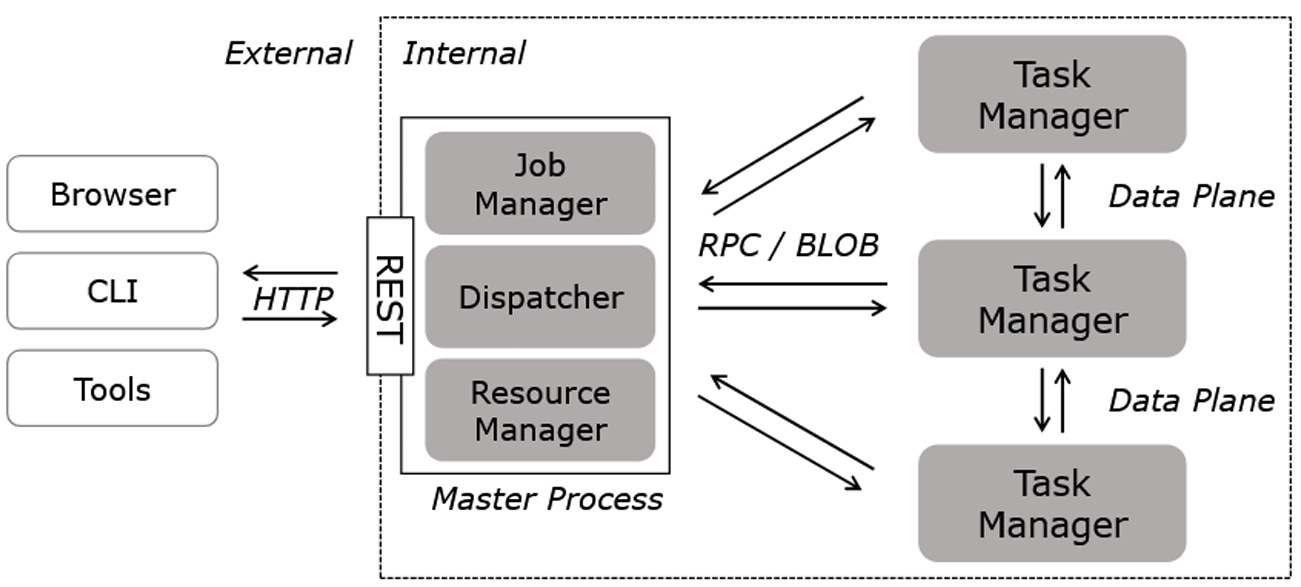
\includegraphics[width=0.9\textwidth]{img/flink_connectivity}
    \captionof{figure}{Metrics exploitation}
\end{center}

Figure 4.28 presents an example of application metrics, allowing visualization of messages that were successfully sent as well as those that were rejected.
It offers an overview of data volumes processed over time, thus facilitating trend analysis over specific periods.

\begin{center}
    \centering
    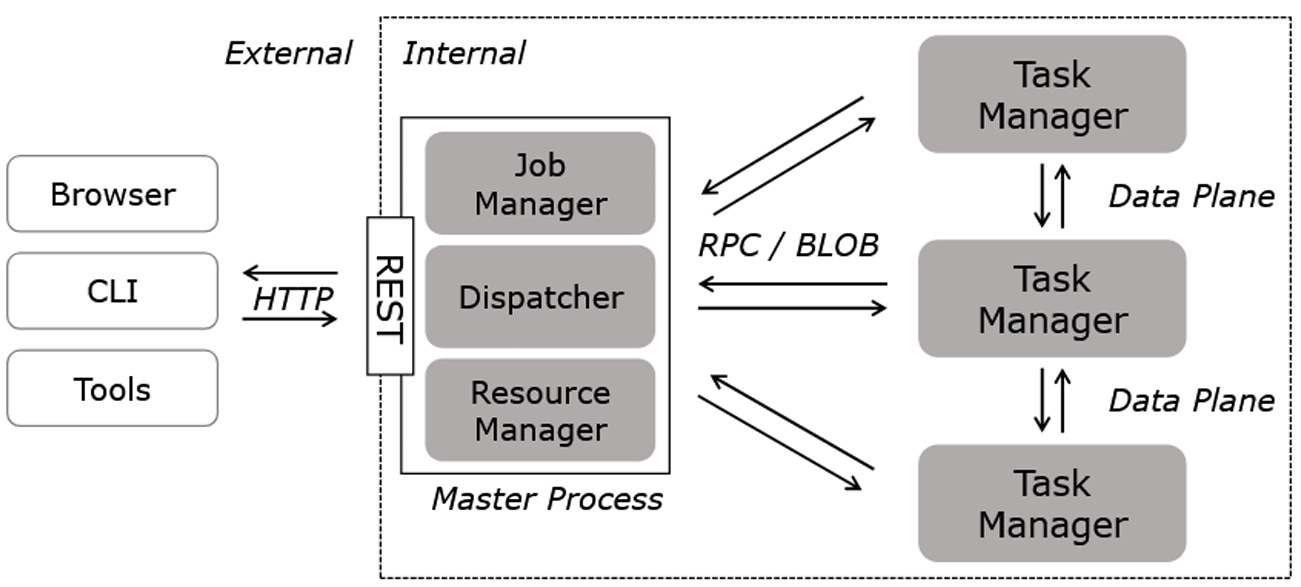
\includegraphics[width=0.9\textwidth]{img/flink_connectivity}
    \captionof{figure}{Application metrics}
\end{center}

Figure 4.29 illustrates system metrics such as JobManager CPU usage, along with other relevant details.
It allows us to investigate whether we are encountering resource utilization issues.

\begin{center}
    \centering
    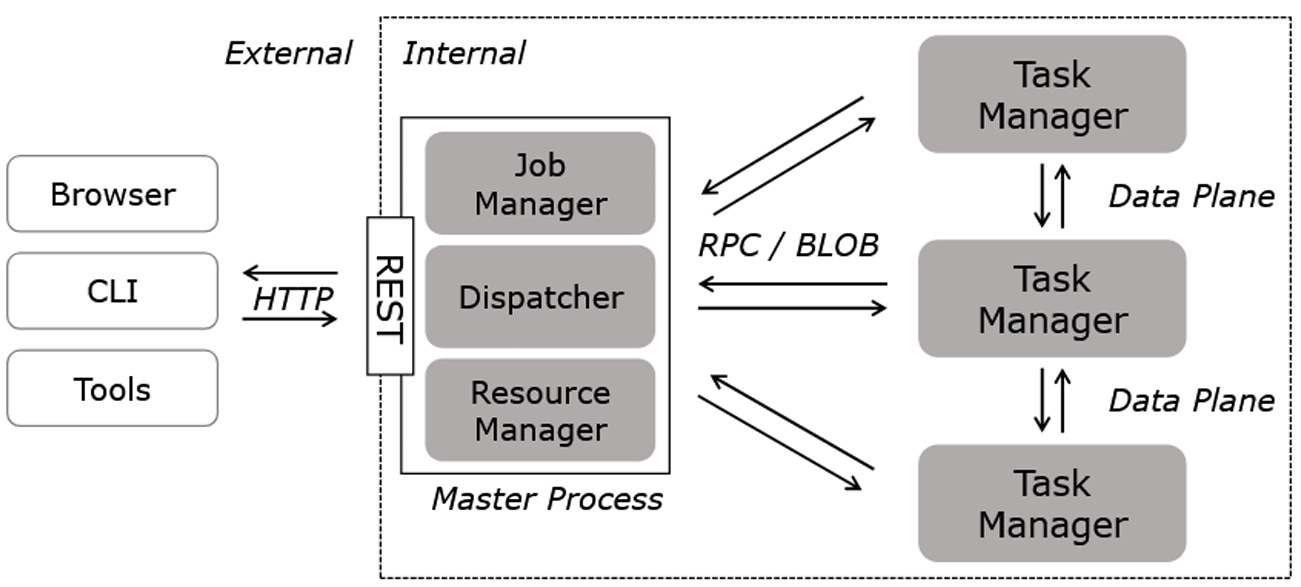
\includegraphics[width=0.9\textwidth]{img/flink_connectivity}
    \captionof{figure}{System metrics}
\end{center}

\section{Continuous integration pipeline}
Figure 4.30 represents the pipeline that triggers each time a commit is made to the main branch (master).
Our pipeline is divided into three stages:

\begin{center}
    \centering
    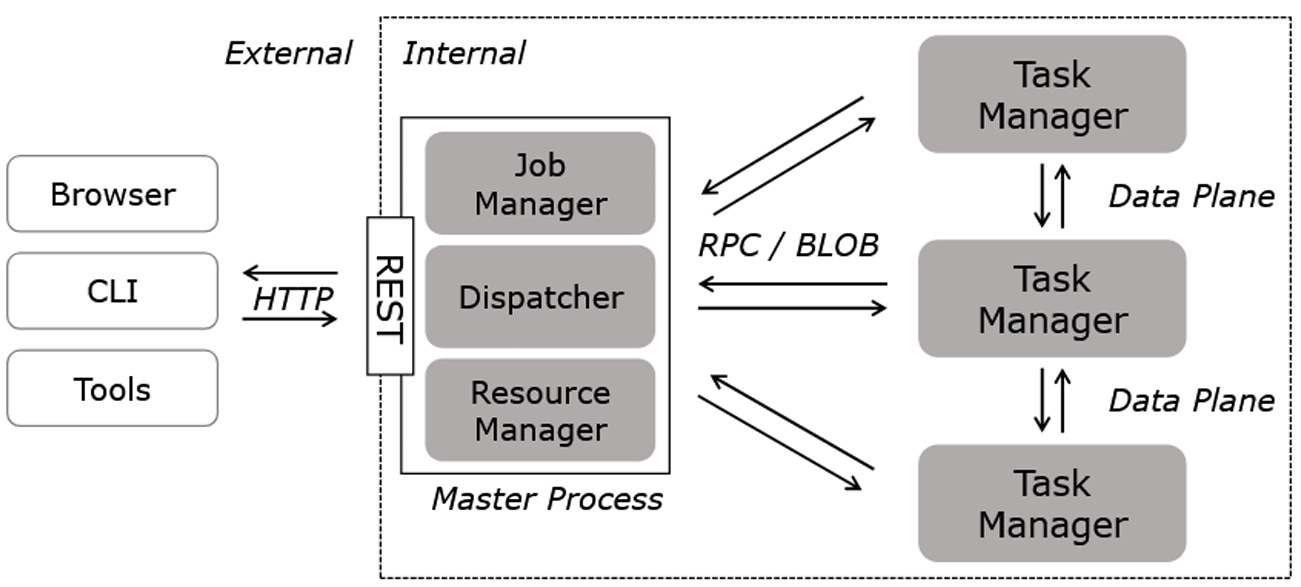
\includegraphics[width=0.9\textwidth]{img/flink_connectivity}
    \captionof{figure}{Continuous integration pipeline}
\end{center}

\begin{enumerate}
    \item \textbf{Build:} It contains a single job bearing the same name as the stage and aims to compile the Java source code. The result is a JAR that will be stored in the job's artifacts. This JAR will be embedded in the Docker image. During this stage, unit and integration tests are executed to ensure that no regression has been introduced.

    \item \textbf{Analysis:} This stage contains two jobs:
    \begin{itemize}
        \item[-] \textbf{Fortify:} is a security-oriented static analysis tool that identifies potential security vulnerabilities in the source code.
        \item[-] \textbf{Sonar:} is a tool dedicated to continuous inspection of source code quality. It offers advanced static code analysis features to identify bugs, vulnerability risks, poor coding practices, and to evaluate test coverage. Its objective is to maintain continuous measurement of code quality.
    \end{itemize}

    \item \textbf{DockerBuild:} This stage includes a single job responsible for building the Docker image. It depends on the build job, which prepares the JAR so it can be integrated into the Docker image, then pushed to the Artifactory. This subsequently allows retrieving the image for deployment.
\end{enumerate}

\section*{Conclusion}
In this chapter, we implemented the solution, consisting of a Flink job performing real-time data processing, as well as its deployment on Kubernetes through the various technologies and software used throughout this work.
